% !TeX spellcheck = ru_RU
% !TEX root = vkr.tex

\section{Экспериментальное исследование}

\subsection{Методология эксперимента}

Эксперименты проводились на трёх платформах. Banana Pi BPI-F3 оснащён процессором SpacemiT K1 (8 ядер RISC-V @ 2.0 ГГц), GPU IMG BXE-2-32 и 16 ГБ LPDDR4-2666. StarFive VisionFive 2 использует процессор JH7110 (4 ядра RISC-V @ 1.5 ГГц), GPU IMG BXE-4-32 MC1 и 8 ГБ LPDDR4-2800. Intel Core i9-12900H имеет 14 ядер (до 5.0 ГГц), Intel Iris Xe Graphics и 24 ГБ DDR5-4800.

Для автоматизации тестирования использовался репозиторий matrix-benchmark~\cite{matrix_benchmark_repo} со скриптами \texttt{benchmark.sh} и \texttt{conf.sh}. Библиотека CLBlast тестировалась в двух вариантах: со стандартными параметрами и после автоматического тюнинга встроенной утилитой \texttt{clblast\_tuner\_xgemm}.

Для MyGEMM выполнялось по 100 прогонов каждой конфигурации, для CLBlast --- по 10 прогонов. Измерялось только время выполнения OpenCL ядра без учёта загрузки данных. Основной размер матриц для сравнения --- $1024 \times 1024$ элементов типа \texttt{float}, для анализа масштабируемости CLBlast использовался диапазон от $512 \times 512$ до $7680 \times 7680$. Стандартное отклонение измерений не превысило 2\% для всех конфигураций.

\subsection{Тестирование библиотеки MyGEMM}

Для тестирования использовались 11 ядер MyGEMM с параметрами, адаптированными под ограничение в 32 потока на рабочую группу для RISC-V платформ. Ядра 1--3 тестировались с параметром TS со значениями 8 и 16 (значение 32 вызывало ошибку \texttt{Invalid work group size}). Для ядер 4--10 использовались комбинации параметров TSM и TSN из множества \{32, 64, 128\} с соответствующими значениями WPTM и WPTN, всего 9 конфигураций для каждого ядра. Ядро 11 тестировалось с фиксированной конфигурацией из реализации clBLAS.

Результаты представлены на рисунках~\ref{fig:perf_bananapi}--\ref{fig:perf_intelxe}. Производительность существенно различается между платформами: Intel выполняет операции за 0.004--0.029 секунд, Banana Pi --- за 0.3--11 секунд (в 75--380 раз медленнее), StarFive --- за 0.5--9 секунд (в 125--225 раз медленнее).

\begin{figure}[H]
\centering
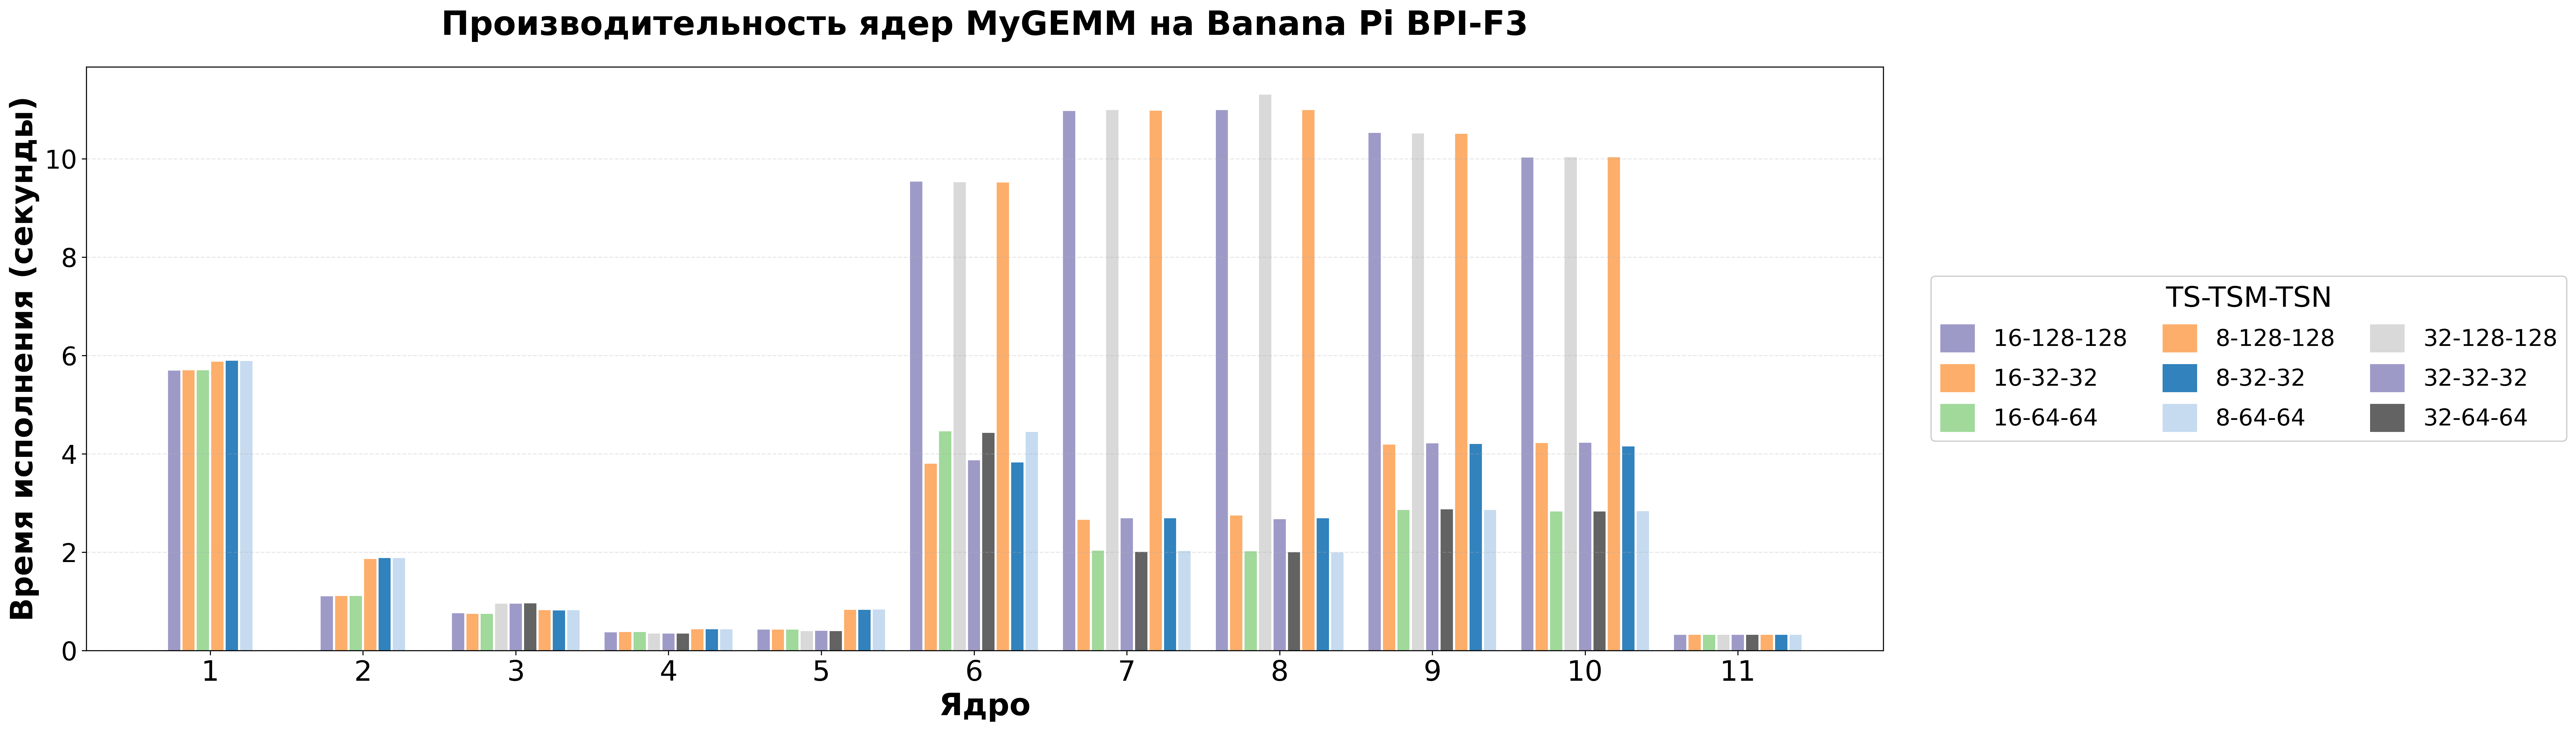
\includegraphics[width=1\textwidth]{figures/banana_pi.png}
\caption{Производительность ядер MyGEMM на платформе Banana Pi BPI-F3}
\label{fig:perf_bananapi}
\end{figure}

\begin{figure}[H]
\centering
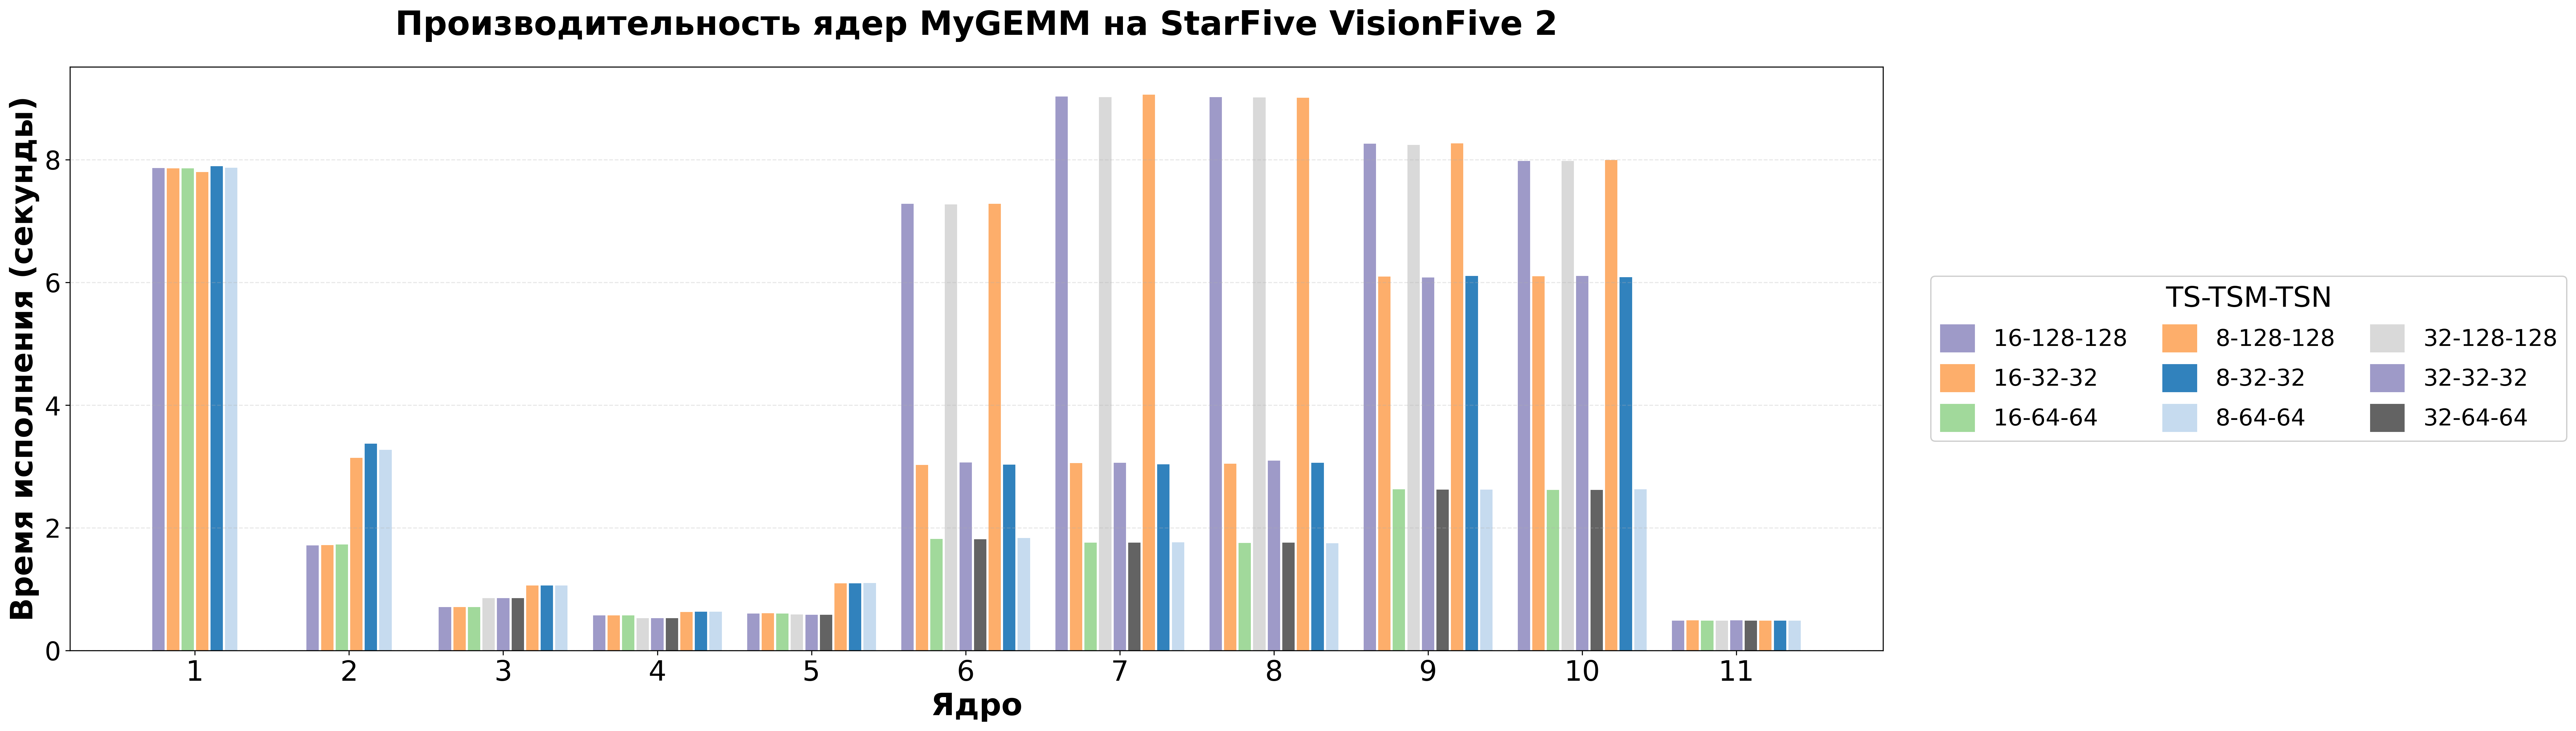
\includegraphics[width=1\textwidth]{figures/starfive.png}
\caption{Производительность ядер MyGEMM на платформе StarFive VisionFive 2}
\label{fig:perf_starfive}
\end{figure}

\begin{figure}[H]
\centering
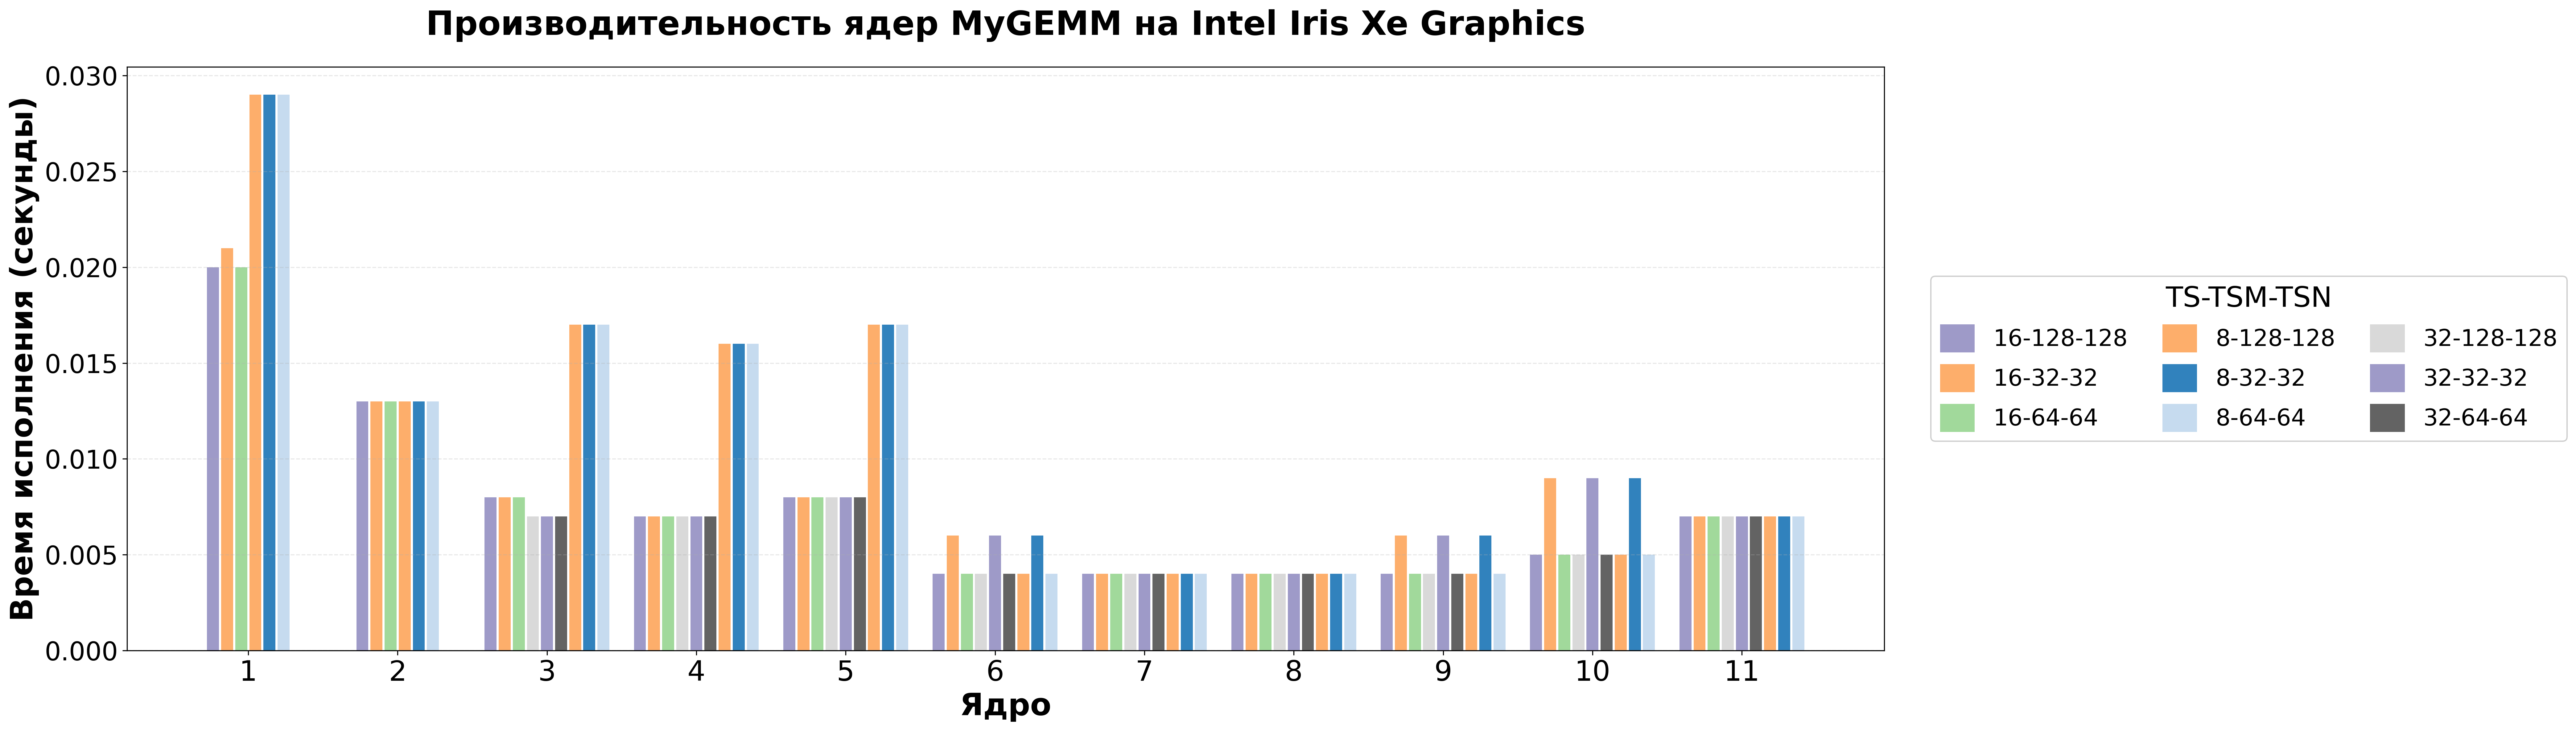
\includegraphics[width=1\textwidth]{figures/intel_xe.png}
\caption{Производительность ядер MyGEMM на платформе Intel Core i9-12900H}
\label{fig:perf_intelxe}
\end{figure}

Ядро 11 показало лучшие результаты на всех платформах: 0.32 секунды на Banana Pi (ускорение в 18.4 раза относительно наивной реализации), 0.49 секунды на StarFive (ускорение в 16.1 раза) и 0.007 секунды на Intel. Ядра 2--5 с использованием локальной памяти дают ускорение в 10--25 раз на RISC-V платформах.

Ядра 6--10 с векторизацией показали низкую производительность: время выполнения 9--11 секунд, что в 10--30 раз медленнее ядер 3--5 и в 600--1000 раз медленнее Intel. Предположительно, это связано с неоптимизированной компиляцией векторных операций \texttt{vload}/\texttt{vstore} в драйверах OpenCL для PowerVR BXE, возможной эмуляцией на CPU или проблемами выравнивания данных.

\subsection{Тестирование библиотеки CLBlast}

CLBlast устанавливалась и тестировалась с использованием скриптов автоматизации из репозитория matrix-benchmark~\cite{matrix_benchmark_repo}. Параметры сборки и тестирования задавались в конфигурационном файле \texttt{conf.sh}, после чего скрипт \texttt{benchmark.sh} автоматически выполнял загрузку исходного кода, сборку библиотеки и тестирование.

Процедура автоматического тюнинга выполнялась отдельно для каждой платформы с помощью встроенной утилиты по документации CLBlast. После завершения тюнинга библиотека тестировалась повторно с использованием того же скрипта \texttt{benchmark.sh} для оценки влияния оптимизации параметров на производительность.

Результаты тюнинга приведены в таблице~\ref{tab:tuning_effect}.

\begin{table}[h!]
\centering
\caption{Влияние автоматического тюнинга CLBlast (время в мс)}
\label{tab:tuning_effect}
\begin{tabular}{|l|r|r|r|r|}
\hline
\textbf{Платформа} & \textbf{Размер} & \textbf{До тюнинга} & \textbf{После} & \textbf{Изм., \%} \\
\hline
\multirow{3}{*}{StarFive} & 512 & 48.14 & 84.54 & +75.6 \\
 & 1024 & 348.72 & 403.23 & +15.6 \\
 & 7680 & 129438 & 129608 & +0.1 \\
\hline
\multirow{3}{*}{Banana Pi} & 512 & 65.34 & 90.14 & +38.0 \\
 & 1024 & 536.75 & 562.21 & +4.7 \\
 & 7680 & 141445 & 141608 & +0.1 \\
\hline
\multirow{3}{*}{Intel Xe} & 512 & 0.67 & 0.68 & +1.5 \\
 & 1024 & 2.24 & 2.18 & -2.7 \\
 & 7680 & 819.14 & 809.12 & -1.2 \\
\hline
\end{tabular}
\end{table}

На RISC-V платформах тюнинг ухудшает производительность: на матрицах 512×512 замедление составляет 75.6\% для StarFive и 38.0\% для Banana Pi. Для размера 1024×1024 ухудшение меньше --- 15.6\% и 4.7\% соответственно. На больших матрицах (7680×7680) изменения минимальны (около 0.1\%). 

На платформе Intel тюнинг даёт небольшое улучшение: 2.7\% для матриц 1024×1024 и 1.2\% для 7680×7680. 

Автотюнер CLBlast формально соблюдает аппаратные ограничения (не превышает лимит в 32 потока), но его эвристики разработаны для GPU с большими рабочими группами (256--1024 потока). В условиях жёстких ограничений RISC-V эти эвристики работают неэффективно. Параметры по умолчанию, вероятно, были вручную настроены для PowerVR BXE, поэтому они лучше результатов автотюнинга.

Рисунки~\ref{fig:clblast_time} и~\ref{fig:clblast_gflops} иллюстрируют эти результаты. Для большинства практических задач с матрицами среднего размера (до 2048×2048) на RISC-V платформах рекомендуется использовать CLBlast без автотюнинга.

\begin{figure}[h!]
\centering
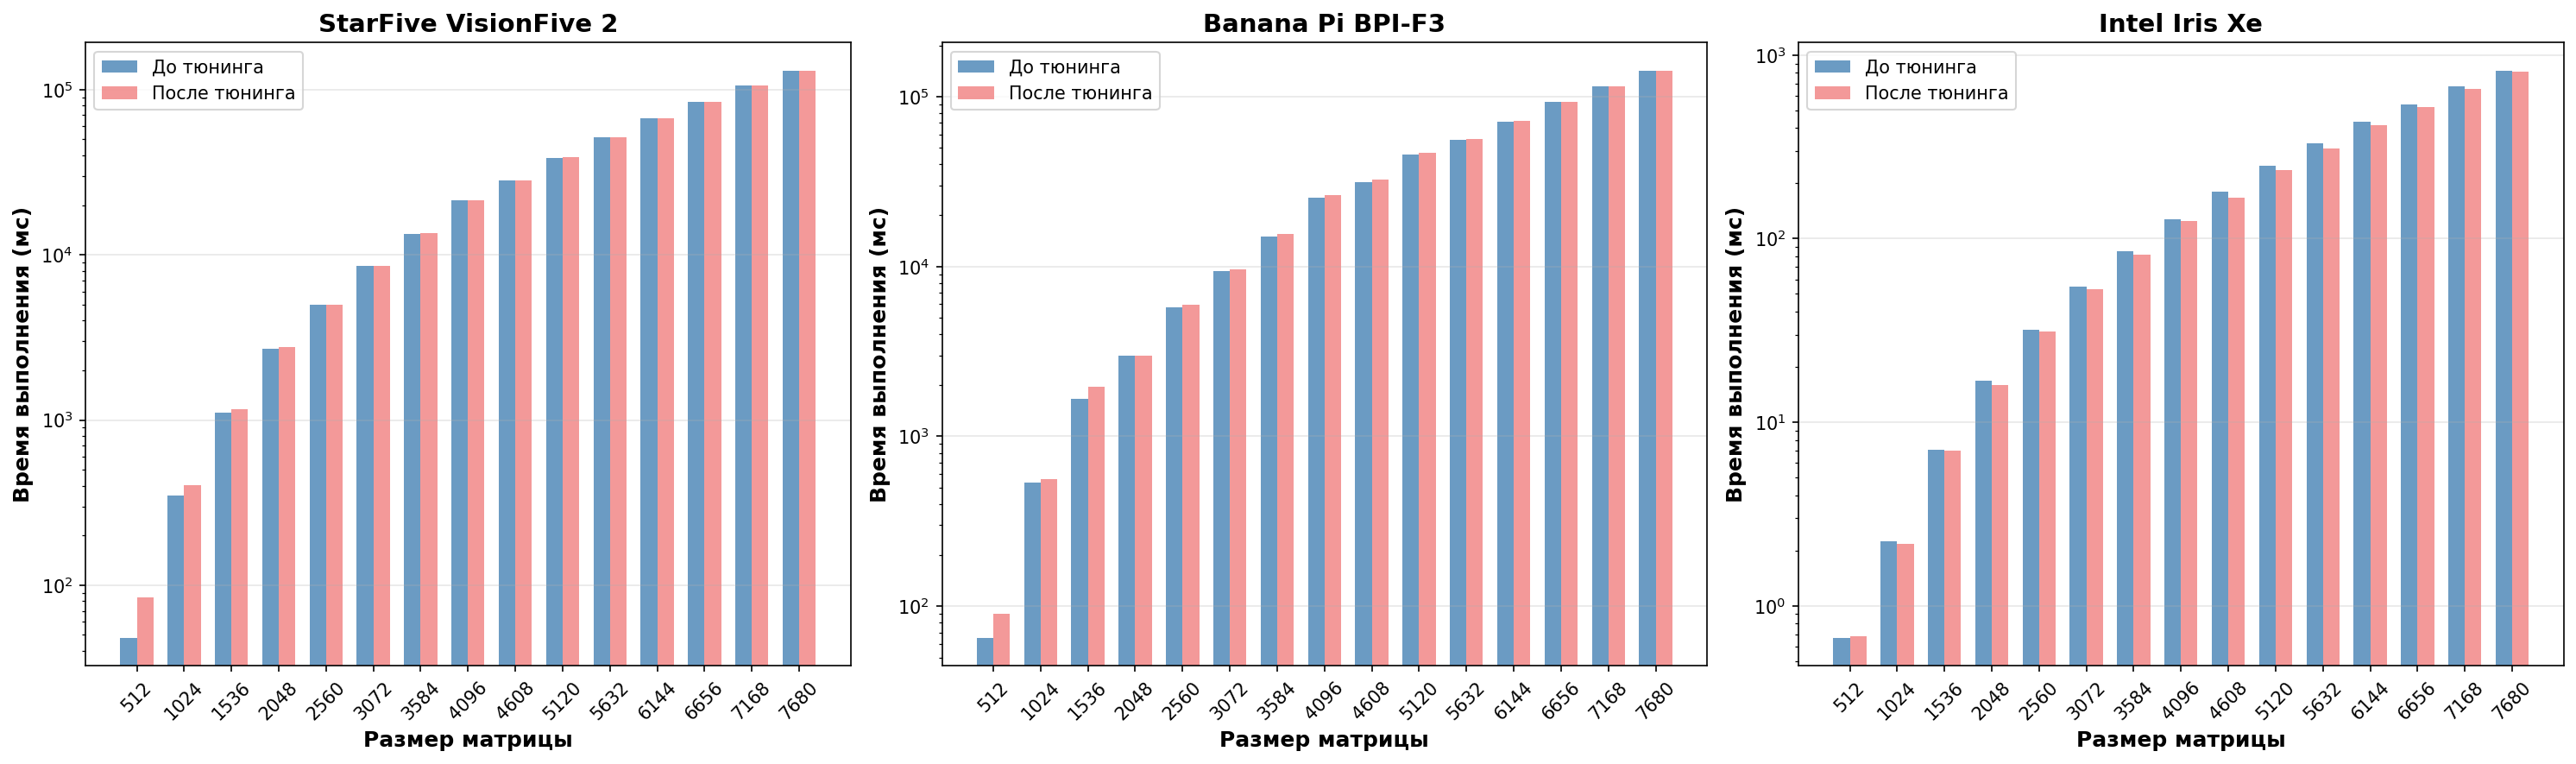
\includegraphics[width=\textwidth]{figures/clblast_time_comparison.png}
\caption{Время выполнения CLBlast до и после тюнинга}
\label{fig:clblast_time}
\end{figure}

\begin{figure}[h!]
\centering
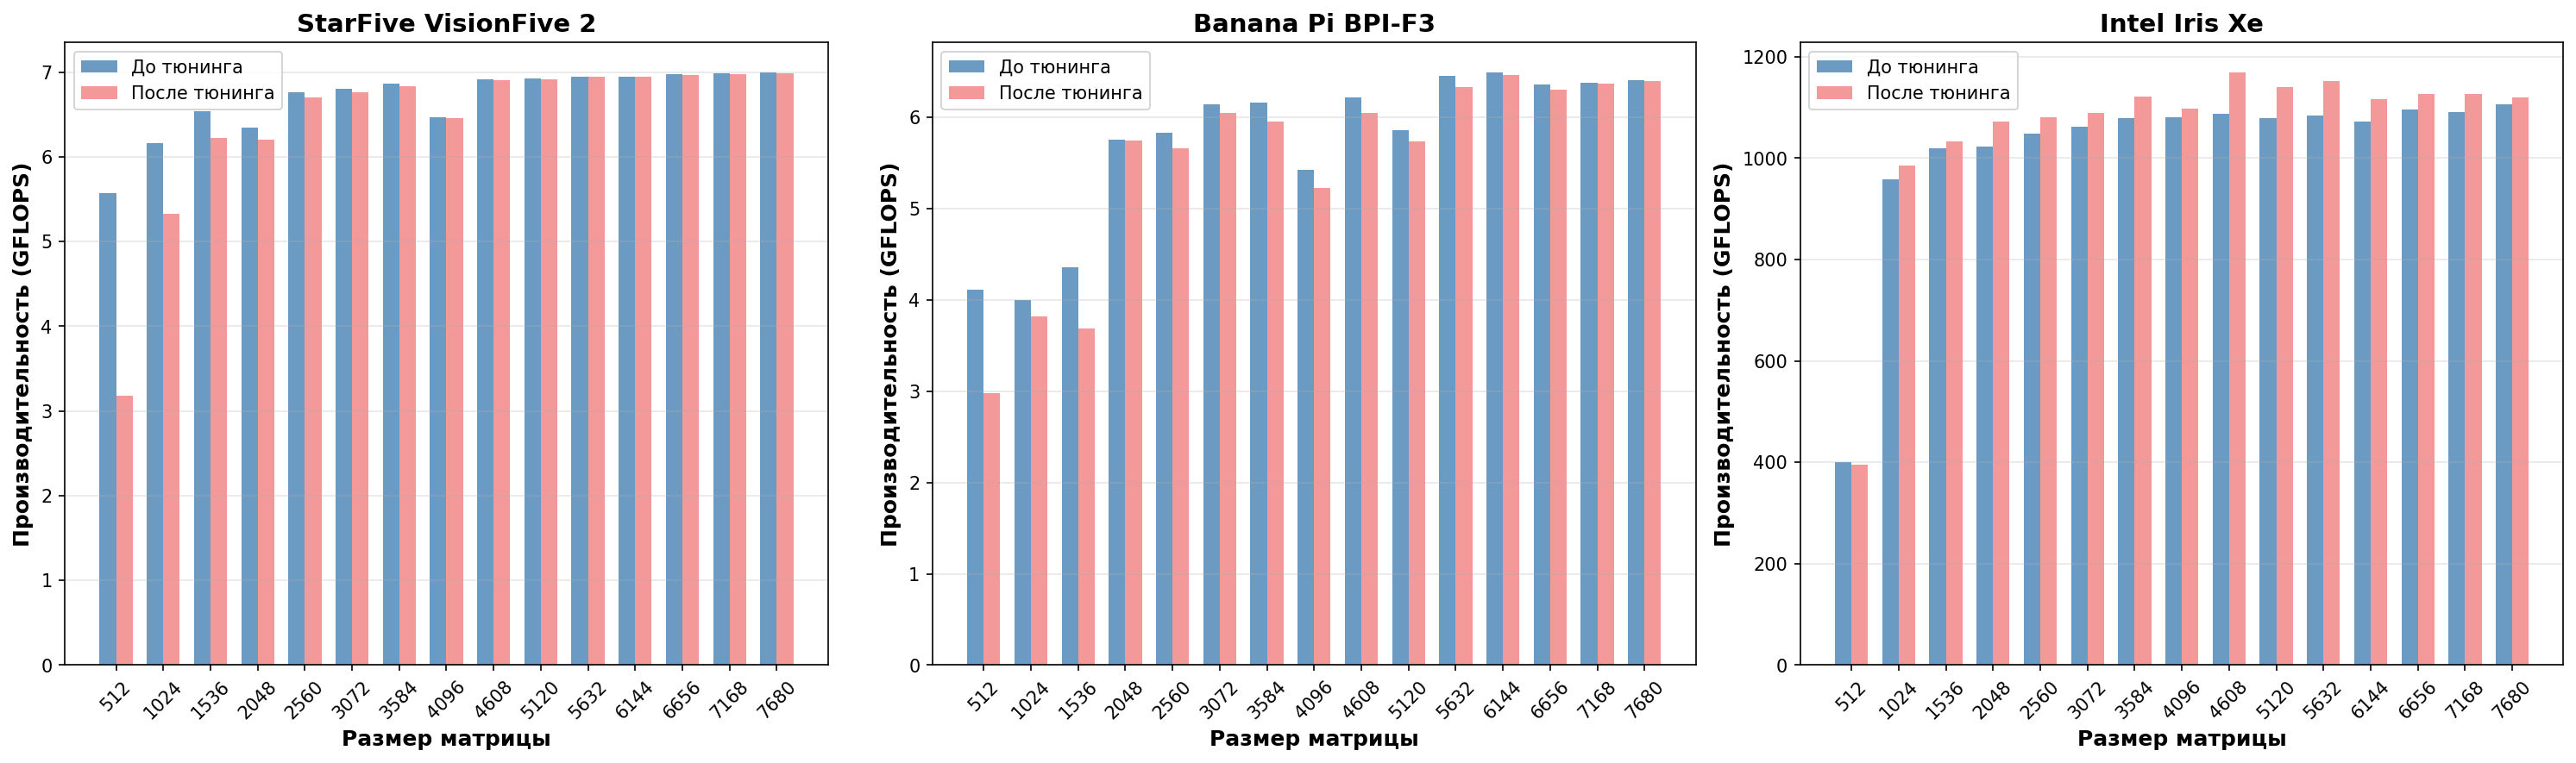
\includegraphics[width=\textwidth]{figures/clblast_gflops.png}
\caption{Производительность CLBlast в GFLOPS}
\label{fig:clblast_gflops}
\end{figure}

\subsection{Сравнение библиотек}

Для матриц 1024×1024 CLBlast с параметрами по умолчанию показывает лучшую производительность. На StarFive время выполнения составляет 0.349 секунды (6.16 GFLOPS), что на 40\% быстрее лучшего ядра MyGEMM. На Banana Pi CLBlast работает за 0.536 секунды (4.01 GFLOPS), уступая MyGEMM на 67\%.

После тюнинга CLBlast на RISC-V платформах замедляется: до 0.403 секунды на StarFive и 0.562 секунды на Banana Pi, что всё ещё быстрее MyGEMM, но существенно хуже исходной конфигурации. Сравнение представлено на рисунке~\ref{fig:clblast_vs_mygemm}.

\begin{figure}[h!]
\centering
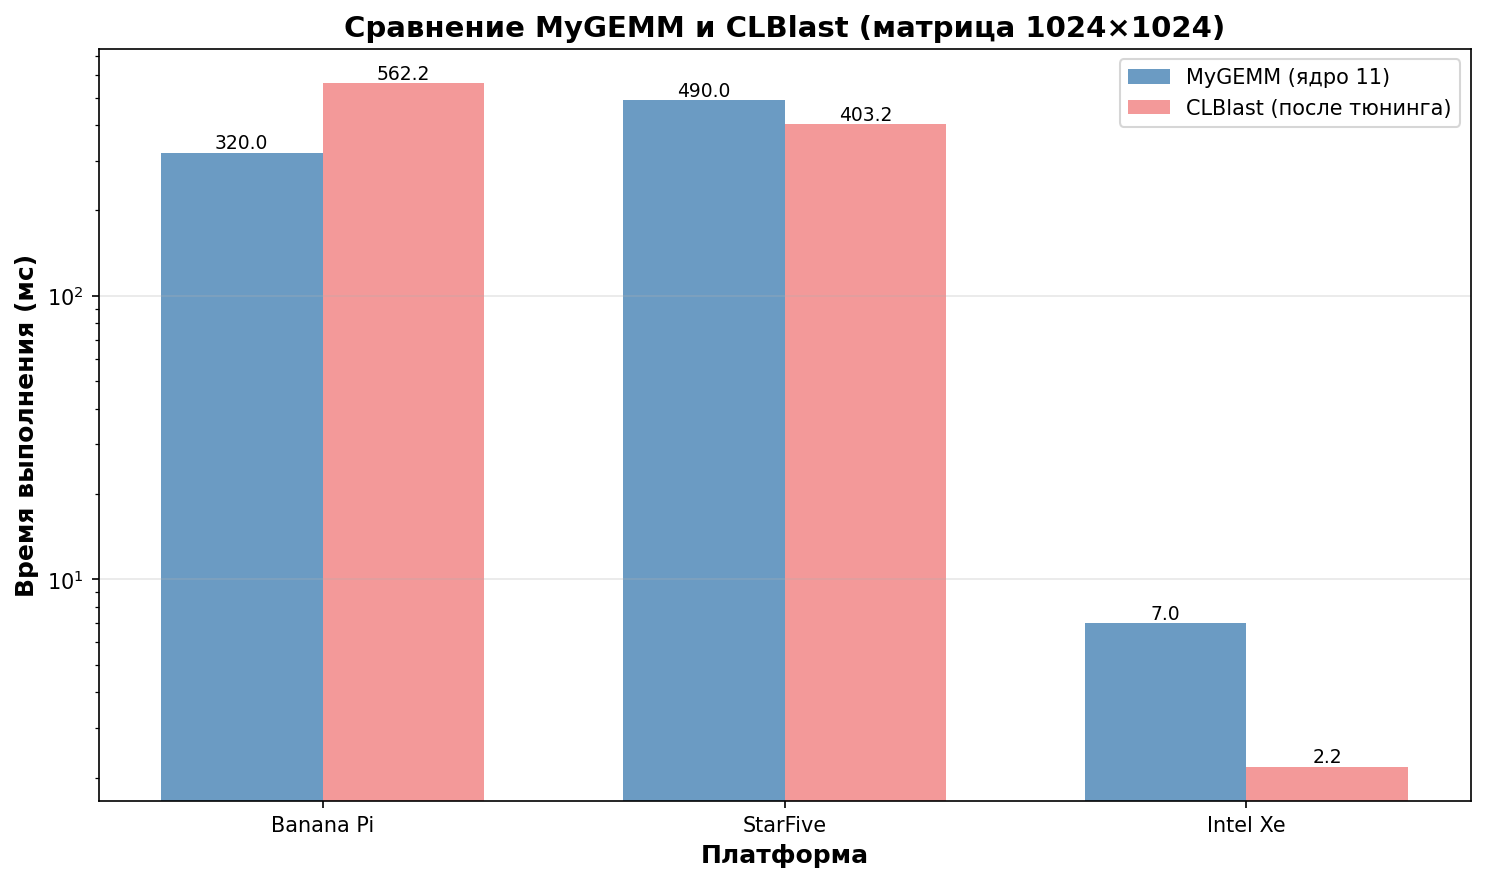
\includegraphics[width=0.8\textwidth]{figures/mygemm_vs_clblast.png}
\caption{Сравнение MyGEMM и CLBlast на матрицах 1024×1024}
\label{fig:clblast_vs_mygemm}
\end{figure}

Обе библиотеки демонстрируют стабильность выполнения со стандартным отклонением менее 2\%. На RISC-V платформах вариативность измерений немного выше, чем на Intel, но остаётся в приемлемых пределах.